%%%%%%%%%%%%%%%%%%%%%%%%%%%%%%%%%%%%%%%%%%%%%%%%%%%%%%%%%%%%%%%%%%%%%%%%%%%%%%%%
% Template for USENIX papers.
%
% History:
%
% - TEMPLATE for Usenix papers, specifically to meet requirements of
%   USENIX '05. originally a template for producing IEEE-format
%   articles using LaTeX. written by Matthew Ward, CS Department,
%   Worcester Polytechnic Institute. adapted by David Beazley for his
%   excellent SWIG paper in Proceedings, Tcl 96. turned into a
%   smartass generic template by De Clarke, with thanks to both the
%   above pioneers. Use at your own risk. Complaints to /dev/null.
%   Make it two column with no page numbering, default is 10 point.
%
% - Munged by Fred Douglis <douglis@research.att.com> 10/97 to
%   separate the .sty file from the LaTeX source template, so that
%   people can more easily include the .sty file into an existing
%   document. Also changed to more closely follow the style guidelines
%   as represented by the Word sample file.
%
% - Note that since 2010, USENIX does not require endnotes. If you
%   want foot of page notes, don't include the endnotes package in the
%   usepackage command, below.
% - This version uses the latex2e styles, not the very ancient 2.09
%   stuff.
%
% - Updated July 2018: Text block size changed from 6.5" to 7"
%
% - Updated Dec 2018 for ATC'19:
%
%   * Revised text to pass HotCRP's auto-formatting check, with
%     hotcrp.settings.submission_form.body_font_size=10pt, and
%     hotcrp.settings.submission_form.line_height=12pt
%
%   * Switched from \endnote-s to \footnote-s to match Usenix's policy.
%
%   * \section* => \begin{abstract} ... \end{abstract}
%
%   * Make template self-contained in terms of bibtex entires, to allow
%     this file to be compiled. (And changing refs style to 'plain'.)
%
%   * Make template self-contained in terms of figures, to
%     allow this file to be compiled. 
%
%   * Added packages for hyperref, embedding fonts, and improving
%     appearance.
%   
%   * Removed outdated text.
%
%%%%%%%%%%%%%%%%%%%%%%%%%%%%%%%%%%%%%%%%%%%%%%%%%%%%%%%%%%%%%%%%%%%%%%%%%%%%%%%%

\documentclass[letterpaper,twocolumn,10pt]{article}
\usepackage{usenix2019_v3}
\usepackage{cancel}
% to be able to draw some self-contained figs
\usepackage{tikz}
\usepackage{amsmath}

% inlined bib file
\usepackage{filecontents}
\usepackage{tikz}
\usepackage{amsmath}
% added to break the urls
\usepackage{xurl} 
% \usepackage{amssymb}
\usepackage{amsfonts}
\usepackage{ifthen}
\usepackage{shadow}
\usepackage{hhline}
\usepackage{tabularx}
\usepackage{fancyhdr}
\usepackage{etoolbox}
\usepackage[T1]{fontenc}
\usepackage{textcomp}
\usepackage{enumitem}
\usepackage{color}
\usepackage{colortbl}
\usepackage{enumitem}
\usepackage{cancel}
\usepackage{bbding}
%\usepackage{cite}
\usepackage{booktabs}
\usepackage{multirow}
\usepackage{tabularx}
% \usepackage{minted}
% \usepackage[ruled,vlined]{algorithm2e}
% \SetKw{Continue}{continue}
% \usepackage{algorithmicx}
% \usepackage{algorithmic}
% \usepackage{algorithm}
% \usepackage{algpseudocode}
% \usepackage{picins}
% \usepackage{minted}
% \hypersetup{draft}
% \usepackage{url}
\usepackage{subcaption}
\usepackage{makecell}

%-------------------------------------------------------------------------------
\begin{filecontents}{\jobname.bib}
%-------------------------------------------------------------------------------
@Book{arpachiDusseau18:osbook,
  author =       {Arpaci-Dusseau, Remzi H. and Arpaci-Dusseau Andrea C.},
  title =        {Operating Systems: Three Easy Pieces},
  publisher =    {Arpaci-Dusseau Books, LLC},
  year =         2015,
  edition =      {1.00},
  note =         {\url{http://pages.cs.wisc.edu/~remzi/OSTEP/}}
}
@InProceedings{waldspurger02,
  author =       {Waldspurger, Carl A.},
  title =        {Memory resource management in {VMware ESX} server},
  booktitle =    {USENIX Symposium on Operating System Design and
                  Implementation (OSDI)},
  year =         2002,
  pages =        {181--194},
  note =         {\url{https://www.usenix.org/legacy/event/osdi02/tech/waldspurger/waldspurger.pdf}}}
\end{filecontents}

\newcommand*\STAIF[0]{VAIF} % In case we want to change this later
\newcommand*\staif[0]{VAIF} % In case we want to change this later
%-------------------------------------------------------------------------------
\begin{document}
%-------------------------------------------------------------------------------

%don't want date printed
\date{}

% make title bold and 14 pt font (Latex default is non-bold, 16 pt)
\title{Automating instrumentation choices for performance problems in distributed applications with VAIF}
% \title{ClaTex: LaTeX as a Service on the Cloud}
\author{Mert Toslali$^{\star}$, Emre Ates$^{\star}$, Alex Ellis$^{\dagger}$, Zhaoqi Zhang$^{\dagger}$, \\
% \email{ates@bu.edu, lsturman@redhat.com, toslali@bu.edu}
Darby Huye$^{\dagger}$, Lan Liu$^{\dagger}$, Samantha Puterman$^{\star}$, Ayse K. Coskun$^{\star}$, Raja R. Sambasivan$^{\dagger}$
% \email{okrieg@bu.edu, acoskun@bu.edu, raja@cs.tufts.edu} 
% \author{%
  \\{$^{\star}$Boston University, $^{\dagger}$Tufts University}
}
\maketitle

%-------------------------------------------------------------------------------
\begin{abstract}
%-------------------------------------------------------------------------------
Developers use logs to diagnose performance problems in distributed
  applications.  However, it is difficult to know a priori where logs
  are needed and what information in them is needed to help diagnose
  problems that may occur in the future.  We present the
  \underline{V}ariance-driven \underline{A}utomated
  \underline{I}nstrumentation \underline{F}ramework (\STAIF{}), which
  runs alongside distributed applications.  In response to
  newly-observed performance problems, \STAIF{} automatically searches
  the space of possible instrumentation choices to enable the logs
  needed to help diagnose them. 
  To work, \STAIF{} combines distributed tracing (an enhanced form of logging) with insights
  about how response-time variance can be decomposed on the
  critical-path portions of requests' traces.  We evaluate \STAIF{} by
  using it to localize performance problems in OpenStack.  We
  show that \STAIF{} can localize problems related to slow code paths,
  resource contention, and problematic third-party code while enabling
  only 3-34\% of the total tracing instrumentation.
\end{abstract}


%-------------------------------------------------------------------------------
\section{Introduction}
%-------------------------------------------------------------------------------


Logs are the de-facto data source engineers use to diagnose
performance problems in deployed distributed applications.  However, it is
difficult to know a priori \textit{where} logs are needed to help
diagnose problems that may occur in the future~\cite{Zhao:2017co,
  Yuan:2012eh, Yuan:2012ws, Mace:2015uh}.  Exhaustively recording all
possible distributed-application behaviors is infeasible due to the
resulting overheads.  As a result of these issues, distributed
applications can contain lots of log statements, but rarely the right
ones in the locations needed to diagnose a specific
problem~\cite{Mace:2015uh, Yuan:2012eh}. New performance problems
cannot be diagnosed quickly because the detailed logs needed to locate
their sources are not present.

Diagnosing problems observed in deployment requires the ability to
customize logging choices during runtime.  Two sets of complementary
techniques allow for such customization: dynamic logging and automated
control of logging choices.  The former allows developers to insert
new logs in pre-defined~\cite{Erlingsson:2011wy,Mace:2015uh,
  Cantrill:2004dtrace} or almost arbitrary locations~\cite{kprobes} of
an application.  But, it can result in high diagnosis times because
engineers must manually explore the vast space of possible logging
choices to locate the source of the problem.  Only after doing so can
they identify the problem's root cause and fix it.

To reduce diagnosis times, researchers have developed automated
techniques to choose the needed logs~\cite{Zhao:2017co,
  ArumugaNainar:2010fx, Zuo:2016et, Liblit:2003ko, Ding:2015td}. However,
they focus on correctness problems, not performance, or are designed
for individual processes, not distributed
applications.  For example, Log20~\cite{Zhao:2017co} helps diagnose
non-fail-stop correctness problems by enabling logs to differentiate
unique code paths.  However, fast code paths need not be differentiated
for performance problems, and slow ones may need additional logs to
further pinpoint the problem source.
Log\textsuperscript{2}~\cite{Ding:2015td} identifies which logs
provide insight into performance problems in
individual processes. Its value is
  diminished for distributed applications because it is unaware of
  slow requests' workflows---i.e., the application processes involved
  in servicing them.

% to store long term, not which ones to enable in the first place.
This paper's goal is to create a logging framework that automatically
enables the logs needed to diagnose performance problems in
request-based distributed applications.  We find that the combination
of three insights about the critical-path sections of requests
workflows, distributed tracing (an enhanced form of logging),
and requests' performance variance makes such a framework possible.

The insights are as follows.  First, in many distributed applications,
requests whose workflows are \textit{expected} to have similar
critical paths should perform similarly~\cite{Sambasivan:2012wv}.  If
they do not---i.e., they exhibit high response-time variance---the
expectation is incorrect, and there is something unknown about their
critical paths.  This unknown behavior may be performance problems,
such as slow functions, resource contention, or load imbalances.
Second, distributed tracing captures graphs (traces) of requests'
workflows with resolution equal to the number of logging points in the
application. (Distributed tracing calls log points tracepoints.)
Third, high response-time variance can be localized to sources of high
variance within critical-path portions of requests' workflow traces,
giving insight into where more tracepoints must be enabled to explain
the unknown behavior.  For problems that manifest as consistently-slow
requests instead of high variance ones, a similar process that focuses
on high-latency areas of critical paths can be used.

We present the design of the \underline{V}ariance-driven
\underline{A}utomated \underline{I}nstrumentation
\underline{F}ramework (\STAIF{}).  \STAIF{} is comprised of a
distributed-tracing infrastructure that allows tracepoints to be
enabled or disabled and control logic that decides where to enable
tracepoints based on the performance-variation insights.  It uses
various search strategies (e.g., binary search) to decide which
tracepoints to enable.  During normal operation, \STAIF{} operates
identically to distributed tracing today and generates traces with a
default level of tracepoints enabled.  When developers must diagnose
why requests are slow, they ``push a button'' and \STAIF{}
automatically explores which additional tracepoints must be enabled to
locate the problem source.  Similar to dynamic instrumentation,
\STAIF{}'s approach reduces the burden of deciding which logs to
enable a priori.  It additionally eliminates the manual effort
required to search the space of possible tracepoint choices.

We implemented two prototype \STAIF{}s for OpenStack~\cite{Openstack}
and HDFS~\cite{HDFS} by modifying their existing tracing
implementations.  In both applications, we find that our prototypes
can enable tracepoints to locate the sources of real and synthetically
injected sources of variance and latency even when only a minimal
number of tracepoints are enabled by default.  We find that many real
sources of variance and latency correspond to bug reports in developer
mailing lists.  Our prototypes only enable 3-37\% of the tracepoints
they could enable to localize these issues.

We present the following contributions.
%
\begin{enumerate}[leftmargin=*]
  \itemsep 0pt
   \item We identify requirements for any logging (or tracing)
   infrastructure must satisfy to address key challenges that limit
   their utility for localizing problems.  We identify insights that
   allow these challenges to be addressed for performance problems
   related to slow code paths, code with unpredictable performance,
   and resource contention.
     
   \item Building on the insights, we present the design of \STAIF{},
     an automated instrumentation framework that combines distributed
     tracing with control logic that automatically enables the
     tracepoints needed to localize new performance problems.
     \STAIF{}'s control-logic components are modular and can be
     applied to different distributed applications instrumented with
     tracing without modifications.  Our \STAIF{} design includes elements
     to make it practically useful: a novel data structure for
     explaining \STAIF{}'s tracepoint decisions to developers and
     mechanisms to limit \STAIF{}'s explorations when resources
     available to tracing are constrained.

   \item We demonstrate the efficacy of our \STAIF{}
     prototype by using them to localize sources of high
     variance and consistently-slow performance in OpenStack.
    %  We believe six of them correspond to real bugs reported on
    %  developer mailing lists.  
    We find that those localized regions correspond to bug reports in developer mailing lists.


\end{enumerate}


%% %---------------------------

%-------------------------------------------------------------------------------
\section{Toward automated logging}
%-------------------------------------------------------------------------------

\textcolor{red}{This section introduces challenges in logging to help diagnose performance problems
and derives requirements that any instrumentation framework should satisfy. 
With the key insights, it describes how these requirements can be met
by combining distributed tracing with control logic that focuses on requests' response-time variance.}

\begin{mycomment}
  1. Shortened the section introduction and removed request/response based app subsection
\end{mycomment}

\subsection{Challenges}
\textcolor{red}{
Past research has identified three challenges with logging for localizing problems, that is, giving developers strong starting points for their diagnosis efforts ~\cite{Kiciman2005a}. 
The challenges are: 
1) No perfect one-size-fits-all logs leading to a tussle between informativeness and cost (e.g., overhead), 
2) Extremely large log search spaces, and
3) Data overload leading to a needle-in-the-haystack problem.
}

We argue that these challenges must be addressed
separately for correctness and performance problems as logging for these two classes have different goals.
Logging for correctness must identify the first divergence from normal execution that
leads to problematic regions in the code ~\cite{ArumugaNainar:2010fx,
Yuan:2012eh, Yuan:2010ww, Zuo:2016et}. 
In comparison, logging for performance must identify regions of the code or resource conditions that lead requests to be slow.

% We describe the challenges below and identify requirements they impose
% on logging frameworks.

% \noindent\textbf{No perfect one-size-fits-all instrumentation leading to
%   a tussle between logging generality and overhead} 

\noindent\textbf{No perfect one-size-fits-all instrumentation.}
\\
Past research has argued that the logs needed to localize the
source of one problem may not be useful for others~\cite{Mace:2015uh,
  Yuan:2012eh, Zhao:2017co, Vef:2018bx}.  
The lack of one-size-fits-all logs leads to a tussle to identify which
log statements are most helpful and should be enabled by default.  For
For example, Zhao et al.~\cite{Zhao:2017co} state that Hadoop, HBase, and
Zookeeper have been patched over 28,821 times over their lifetimes to
add, remove, or modify static log statements embedded in their code.
They also point out that the 2,105 revisions that modify logs'
verbosity levels reflect the tussle between a desire to balance
overhead and informativeness of log statements.
This challenge results in the following requirement: 
\begin{description}%[leftmargin=*]
    \itemsep 0 pt
  \item[\textit{R1}] \textit{Logging frameworks must allow logs to be
    enabled selectively by developers during runtime or must
    automatically enable logs in response to problems observed during runtime.}
  \end{description}


  \noindent\textbf{Extremely large logging search spaces.}
\\
Assume a distributed application that allows log points to be enabled
 at every function's entry, exit, and exceptional return. (This
is similar to the distributed applications used by Mace et
al.~\cite{Mace:2015uh} and Erlingsson et
al.~\cite{Erlingsson:2011wy}.)  Here, the possible locations where log
statements can be enabled is a function of the number of procedures in
the applications' code base and the number of machines on which the
application executes.  Even modestly-sized distributed applications
can have search spaces with 100s or 1000s of possible log points.

To address this scalability challenge, we refine \textit{R1} to
require logging frameworks to automatically enable tracepoints.  We
add a requirement stating that frameworks must
automatically narrow down the search space when exploring new
problems.

\begin{description}%[leftmargin=*]
    \itemsep 0 pt
  \item[\textit{R2}] \textit{Automated Logging frameworks must 
    be capable of narrowing down the search space when exploring what
    logs are needed to localize a newly-observed problem.} 
  \end{description}


  \noindent\textbf{The needle-in-a-haystack problem.}
  \\
Existing logging infrastructures capture voluminous amounts of data.
For example, Facebook's Canopy, a distributed-tracing infrastructure
captures 1.16 GB/s of trace data and individual traces contain
1000s of tracepoints~\cite{Kaldor:2017gp}.  Problem diagnosis, even
when the needed instrumentation is present, can be trying to
find a needle in a haystack~\cite{Rabkin:2013wy}.

\textcolor{red}{
  This challenge is partially addressed by \textit{R1} and \textit{R2}.  
}
  To avoid the needle-in-haystack
problem for cases where there may be multiple problems in the
application simultaneously, we add the following requirement.

%\vspace{-0.1in}
\begin{description}%[leftmargin=*]
  \itemsep 0 pt \item[\textit{R3}] \textit{Automated logging
  frameworks must be capable of explaining their logging decisions.}

\end{description}


\subsection{Key insights}
\label{sec:motivaton:insights}

We discuss insights that let us address the requirements and
discuss how the requirements are addressed next.

The first insight is that in many distributed applications, requests
with similar critical paths---i.e., requests that are processed
similarly by the distributed application---will have similar response
times.  An existing use of this insight involves using separate
performance counters for different request types or API calls, such as
\textsc{read}s and \textsc{get attributes} in a distributed-storage
application.  Separate counters are used because there is an
expectation that requests of different types will have very different
critical paths and thus have different response times.

The second insight is that distributed
tracing~\cite{Sambasivan:2016bo, Parker, Shkuro}, which is an enhanced
form of logging, can identify requests' critical paths with resolution
equal to the amount of tracing instrumentation present.  This is
because it records graphs (called \textit{traces}) of requests
workflows.  Today, distributed tracing is becoming increasingly
popular and an ever growing number of distributed applications are
being instrumented with it~\cite{HDFS, CockroachDB, Weil:2006ti,
  Openstack, Kaldor:2017gp, Sigelman:2010uj, Mace2017survey}.

This insight combined with the previous one means that that if
requests' whose workflow traces have identical critical paths
\textit{do not} perform similarly---i.e, their response time variance
is high---there is some unknown behavior that is not captured in their
traces.  This behavior may represent performance problems, such as
slow code paths or functions executing, differences in resources used
or available to requests, poorly-written algorithms that
unintentionally increase variance, or third-party code with
unpredictable performance.

The third insight is that the law of total
variation~\cite{stats_textbook} can be applied to traces of requests'
critical paths.  For a set of requests whose trace critical paths
appear identical as per the enabled tracepoints, this equation can be
interpreted as follows.  The variance of requests' response times is
the variance of the latencies of their critical-path trace edges plus
their covariances.

%This law states that the variance
%of a sum of random variables is the same as the sum of their variances
%plus their pairwise covariances. 

This insight means that we can identify areas in the codebase in which
unknown behavior resides by identifying the edges of requests'
critical-path traces that contribute most to the variance.  The
unknown, potentially problematic behavior resides within the code
regions that execute between the tracepoints that form these edges.


\subsection{Addressing the requirements}
\label{sec:motivation:guiding_principles}

Based on the insights, the requirements can be satisfied for many
classes of performance problems by combining two technologies.  The
first is a distributed-tracing infrastructure that allows tracepoints
to be selectively enabled or disabled during runtime.  The second is a
control mechanism for distributed tracing that automatically enables
tracepoints and considers key/value pairs exposed in them
to \textit{explain} variance as per the insights above.  
The control logic also includes additional principles to diagnose problems that result
identical critical paths having low variance but are very slow and to
explain its decisions.
\begin{mycomment}
  1. Shortened the section introduction by removing second intro paragraph.
\end{mycomment}

% \textcolor{red}{The control
% logic includes additional principles to diagnose problems that result
% identical critical paths having low variance but are very slow and to
% explain its decisions.  We describe the principles of this control
% mechanism below.  We use the term critical-path traces to refer to the
% critical path portions of requests workflows.  We define identical
% critical path traces as those which execute the same tracepoints in
% the same order and whose nodes have identical names.}

%\input{table_requirements}

\noindent\textbf{Principle \#1} Identify requests whose traces exhibit
identical critical paths with high response-time
variance. Identify edges of their traces' critical paths that
contribute most to the variance.  Enable additional tracepoints in
the code regions corresponding to these areas.

Principle one differentiates slow code paths from fast ones and/or
isolates code with unpredictable performance.  It addresses
\textit{R1: enable tracepoints (logs) automatically in response to
  problems} and \textit{R2: narrow down the search space}.

%observed during runtime

This principle is a direct application of the law of total variation
to critical-path traces.  Applying this law narrows down the search
space to tracepoints that can execute between the critical-path trace
edges that contribute most to response-time variance (\textit{R2}).
Enabling some tracepoints in this area adds them to future traces,
either differentiating critical-path traces further to separate fast
ones from slow ones or further isolating areas from which high
variance arises.

%Such variance may be due to black-box
%third-party code, problematic algorithms, or code areas that do not have
%sufficient instrumentation to distinguish different behaviors.%

Iteratively applying this principle until requests with identical
critical-path traces exhibit low response-time variation or until no
additional tracepoints can be enabled accomplishes the
following.  \textit{1)} It sufficiently differentiates fast critical
paths from slow ones or
\textit{2)} isolates high variance coming from black-box third-party
code, problematic algorithms, or differences in resource
usage/availability (\textit{R1}).

% \textit{Example of differentiating slow critical paths from fast ones}:
% Figure~\ref{fig:differentiating_workflows} shows three groups of
% identical critical-path traces from a distributed-storage system,
% similar to Ceph~\cite{Weil:2006ti} or HDFS~\cite{HDFS}.  Nodes
% indicate tracepoint names and edges indicate happens-before
% relationships.  Edges are annotated with distributions of edge
% latencies.  In Figure~\ref{fig:differentiating_workflows_undiff}, the
% response-time variance of \textsc{read} requests with identical
% critical-path traces is high.  The figure shows that the trace edge
% spanning storage node accesses is the dominant contributor to
% response-time variance.
% Figure~\ref{fig:differentiating_workflows_cache_hit}
% and~\ref{fig:differentiating_workflows_cache_miss} shows that enabling
% tracepoints to differentiate cache hits from misses distinguishes fast
% critical paths (cache hits) from consistently slow ones.  (The figures
% show normal distributions, but our principles hold for arbitrary ones.) 

% \input{fig_differentiating_workflows}

% 
% \textit{Example of isolating high variance due to third-party code}:
% Figure~\ref{fig:isolating_variance_third_party_initial} shows that the
% response-time variance of \textsc{directory list} requests with
% identical critical-path traces is high.  The figure shows that the
% trace edge spanning the metadata server, which stores directory
% information, is the dominant contributor to the overall variance.
% Figure~\ref{fig:isolating_variance_third_party_zoomed} shows that
% enabling tracepoints within the metadata server eventually reveals
% that the variance emanates from a third-party database that is storing
% the directory info.

% \input{fig_isolating_variance_third_party}

%\input{fig_workflows}

%%%%%%%%%%%%%%%%%%%%%%%%%

\noindent\textbf{Principle \#2} Identify requests whose traces have
identical critical paths, have low variance, but have high response
times (i.e., are \textit{consistently slow}).  Identify critical-path
trace edges that are dominant contributors to response times and
enable tracepoints in the code regions corresponding to
these areas.

Principle two localizes problems due to slow functions. It addresses
\textit{R1: automatically enable instrumentation} and \textit{R2:
  narrow down the search space}.  It is needed because principle one
identifies slow critical paths, but does not localize slow performance
to specific code areas.  It is similar to the first principle except
it focuses on response times and edge latencies directly instead of
variance.

% \textit{Example}: Requests corresponding to the critical path traces
% in Figure~\ref{fig:differentiating_workflows_cache_miss} have low
% variance but have high response times.  The majority contributor to
% response times is the edge between the \texttt{cache\_miss} tracepoint
% and the \textit{SN\_end} tracepoint.  Iteratively isolating
% dominant contributors to overall response times and enabling
% tracepoints in these areas eventually identifies the function(s) that
% contribute most to response times.

%encapsulating file
%accesses are the dominant cause of the observed latency as shown in
%Figure~\ref{}.


%%%%%%%%%%%%%%%%%%%%%%%%%

\noindent\textbf{Principle \#3} Identify requests whose traces exhibit
identical critical paths with high variance in their
response times.  Identify which key/value pairs exposed by
already-enabled tracepoints correlate highly with requests' response
time.  Augment tracepoint names with these keys and ranges of their
values or directly surface them to developers.

Principle three localizes problems related to resource
usage/availability.  It also differentiates slow critical paths from
fast ones when keys' values record how much work requests must perform
(e.g., read/write sizes in a storage system).  It is an enhancement to
Principle one in that it explores reasons for variation that are not
due to differences in critical paths themselves, but rather due to
external factors at the time of requests' execution \text{red}{(e.g., resource contentions)}.

% \textit{Example}: In our example, OpenStack \textsc{CREATE\_VM} requests, which exhibit high variance.
% The VM\_build\_start function contributes most to variance.  Augment
% the ``mutex\_queue\_length'' key and ranges of its values (e.g., 0-5,
% 6-10, > 10) differentiates critical paths as per their queuing times.
% This localizes the problem to high resource contention in this area.


\noindent\textbf{Principle \#4} Maintain a history of the tracepoints
enabled on behalf of high variance or consistently-slow performance
along with the statistics that motivated these decisions.  This
principle allows the framework to explain why it made the decisions it
did to localize problems (\textit{R3}).


\noindent\textbf{Contrast to related work} Many logging frameworks do not
automatically enable logs or tracepoints~\cite{Erlingsson:2011wy,
Mace:2015uh} (\cancel{R1}) or are designed to automatically enable
instrumentation for fail-stop correctness problems
only~\cite{ArumugaNainar:2010fx, Yuan:2012eh, Yuan:2010ww, Zuo:2016et,
Zhao:2017co}.  Log2~\cite{Ding:2015td} partially addresses \textit{R1}
and \textit{R2} by deciding which already-enabled logs to persist in
storage, not which ones to enable in the first place.  It cannot
explain its decisions in terms of requests' performance (\cancel{R3})
because it is oblivious to requests' workflows or critical paths.
Some logging frameworks~\cite{Zhao:2017co} generically enable logs to
differentiate unique code paths.  This approach is neither sufficient
nor necessary for performance diagnosis.  It is insufficient because
additional logs may be needed to identify where on a code path a
problem lies; it is not necessary when code paths are fast and need
not be differentiated.



%-------------------------------------------------------------------------------
\section{Vision}
%-------------------------------------------------------------------------------

\STAIF{} is an automated instrumentation framework that combines
distributed tracing and control logic based on the principles.  It is
deployed alongside running distributed applications.  In normal
operation, \STAIF{} operates identically to existing distributed
tracing, generating traces using tracepoints that developers wish to
have always on.  These tracepoints may be ones developers have found
useful in the past or ones used for use cases other than performance
diagnosis, such as correctness.  When new performance problems occur,
developers can use \STAIF{} to automatically enrich traces with the
additional tracepoints needed to localize them.

\STAIF{} localizes problems due to slow code or those with
unpredictable performance (high variance).  Such unpredictability may
emanate from areas of the application itself, third-party code the
application uses, or from areas of the application that could benefit
from additional tracing instrumentation. \STAIF{}
also explores whether key/value pairs exposed in tracepoints explain
high variance.  It allows developers to specify important keys that
they suspect will explain variance and bin ranges for them.  \STAIF{}
will augment tracepoint names with these keys if they explain
variance.  It will surface other keys whose values explain variance in
its output.

Like manual dynamic-instrumentation
approaches~\cite{Erlingsson:2011wy, Mace:2015uh}, \STAIF{} frees
developers from the tussle between generality and overhead.  Unlike
manual approaches, it also frees them from having to search the space
of tracepoint choices to enable additional ones.  When enabling
instrumentation, \STAIF{} works in a continuous cycle.  At each
iteration, it uses the principles to hypothesize (guess) which
tracepoints should be enabled next within a high variance or slow area
of the application.  It uses the results of previous hypotheses to
guide future ones.  It uses a novel data structure, called
the \textit{hypothesis forest}, to explain the results of its
hypotheses to developers.  \STAIF{}'s analyses are most useful for
on-path problems.  It also provides value for off-path problems by
identifying the critical-path areas most affected by them.

%
\mert{
  1. Removed last paragraph here (of discussions)
}
% The rest of this section describes \STAIF{} in more detail.  
% Our discussions are agnostic to whether tracepoints are enabled or
% disabled using dynamic instrumentation~\cite{Erlingsson:2011wy,
% Cantrill:2004dtrace, Mace:2015uh} or by modifying existing tracing
% infrastructures' tracepoints to execute conditional checks before
% emitting tracepoint records.  We assume tracepoints are uniquely
% addressable.  Some methods for addressing them include using: their
% names (as done for Linux kernel logs); hashes of their names and their
% keys (if names are not unique); an external registry that assigns
% addresses to tracepoints.  We assume unique names from now on.

\subsection{Design}
Figure~\ref{fig:staif_design} shows \STAIF{}'s design, which builds
upon existing distributed tracing.  It consists of a
control plane and an instrumentation plane.  Components in the
\textit{control plane} implement the control logic whereas
those in the \textit{instrumentation plane} implement the control
logic's hypotheses or provide custom information about the
application.

\STAIF{} works in a continuous loop, which is shown in \textit{red}
in the figure.  At each iteration, \STAIF{}'s instrumentation-plane
components gather new critical-path traces (
\includegraphics[scale=0.5, trim=-0 0.3cm 0 0]{figures/marked_A.pdf} in the figure).
The control-plane components examine them to identify hypotheses of
which tracepoints should be enabled next and which key/value pairs
additionally explain high variance (
\includegraphics[scale=0.5, trim=-0 0.3cm 0 0]{figures/marked_B.pdf}).  Hypotheses are sent to
the instrumentation plane components (
\includegraphics[scale=0.5, trim=-0 0.3cm 0 0]{figures/marked_C.pdf}), which enable the
relevant tracepoints and the cycle repeats. \STAIF{}
pauses its explorations if any of the tracing agents' queues are
congested.  This prevents cases in which \STAIF{} does not observe the
effects of new hypotheses because tracepoints records were dropped.

\begin{figure}[tb]
    \centering
    % \vspace{-0.1cm}
    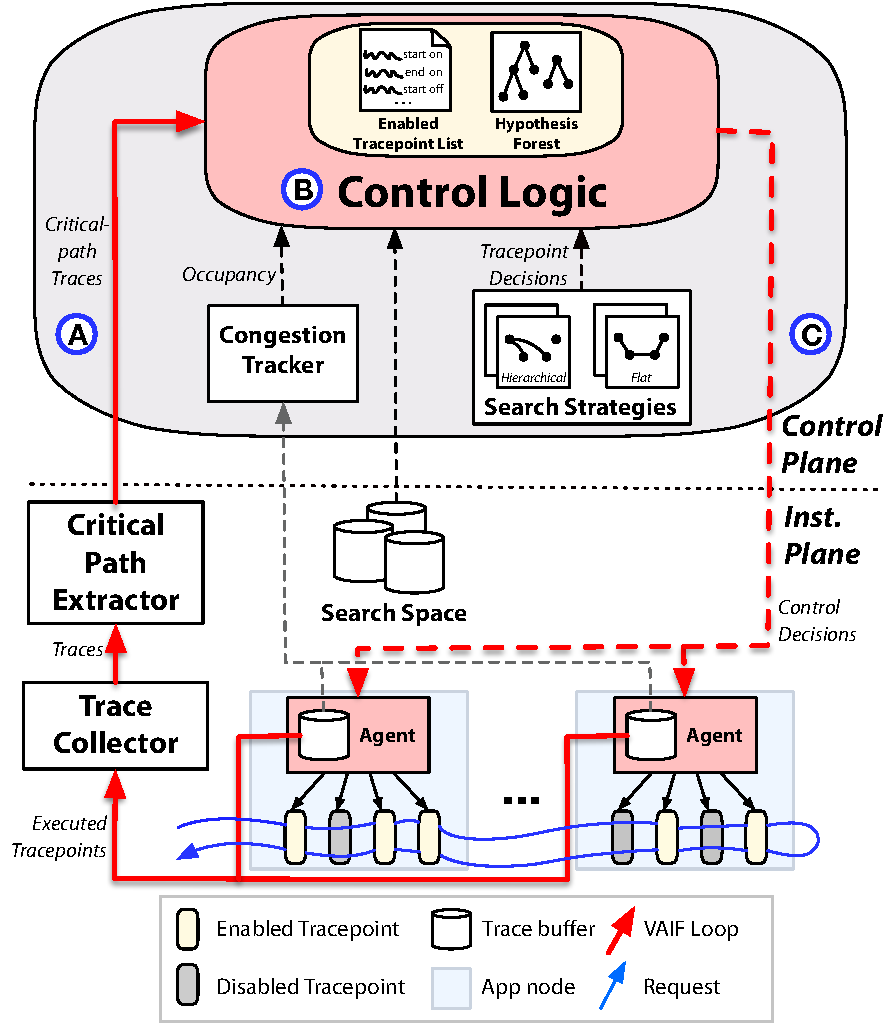
\includegraphics[width=\columnwidth]{figures/fig_staif_design.pdf}
    % \vspace{-0.8cm}
  
    \caption{\STAIF{} design. The thick red line shows \STAIF{}'s
      continuous loop.  Solid lines are traces/tracepoints and dashed
      lines are control signals.  A generic distributed application
      instrumented with tracing is shown in the instrumentation plane.}
    
    \label{fig:staif_design}
     \vspace{-0.2in}
  \end{figure}


  \subsubsection{Components}
  \label{sec:design:components}
%   \hfill\\
  \noindent\textbf{Control plane} The control plane consists of the
  control logic, two search strategies for deciding which tracepoints to
  enable in high-variance or slow areas, and a congestion tracker that
  periodically receives queue occupancies from tracing agents.  The
  search strategies are designed to be generically applicable to many
  distributed applications.  The congestion tracker informs the control
  logic when any tracing agents' queues are in danger of being
  congested, which we define as over 50\% occupancy.  We use this
  conservative definition because \STAIF{} does not know how many times
  tracepoints will execute once enabled.  The control plane also
  maintains important state: a global list of tracepoints that have been
  enabled by \STAIF{}{} and the hypothesis forest.
  
  \STAIF{}'s control-plane components are modular and intended to
  be used with different distributed applications and/or
  tracing infrastructures without modifications.
  
  \noindent\textbf{Instrumentation plane} The instrumentation plane
  consists of an application instrumented with tracing, a critical-path
  extractor that extracts critical-path portions from traces and sends
  them to \STAIF{}'s control-plane components, and a search space that
  describes the application's tracepoints.  The critical-path extractor
  works by identifying the highest-latency trace path from the
  tracepoint indicating request reply to that indicating request start.
  Concurrency and synchronization may result in multiple paths for a
  single trace, each with different latencies.  The search space names
  all of the tracepoints in the distributed application, including the
  keys that will be used in grouping.  It also lists
  concurrency/synchronization tracepoint names as these must be enabled
  for critical-path extraction.
  
  Legacy instrumentation-plane components require modifications to be
  used with \STAIF{}.  First, the tracing
  infrastructure's libraries must allow tracepoints to be selectively
  enabled or disabled during runtime.  They must also let developers
  specify which tracepoints should be considered always on. Second,
  tracing agents co-located with processes must report queue lengths and
  receive updates about which tracepoints to enable or disable. Third,
  tracing infrastructures must preserve happens-before relationships
  between tracepoint records to allow critical paths to be
  extracted. This can be done by exposing APIs to capture them directly
  (as done by X-Trace~\cite{Fonseca:2010vn, Mace:ui},
  Canopy~\cite{Kaldor:2017gp}, and Stardust~\cite{Sambasivan:2011vw}) or
  by learning them over a large number of traces (as done for traces
  that preserve only hierarchical caller/callee relationships, such as
  Dapper~\cite{Mann:2011vf} and Artillery~\cite{Chow:2014ts}).
  
  \vspace{-0.05in}
  \subsubsection{Usage}
  \label{sec:design:init}
  \hfill\\
  \noindent\textbf{Starting \STAIF{}'s exploration} \STAIF{} takes 
  two inputs to start its explorations.  The first is the application
  search space.  The second is a list of tracepoints corresponding to start
  of execution of request types (or endpoints) that are experiencing
  problems.  (We assume tracepoints that name the corresponding replies
  can be programmatically derived otherwise, they would need to be
  provided as well.)
  
  \STAIF{} also takes as input two optional parameters.  
  The first is a threshold for identifying groups of critical-path
  traces that exhibit high variance, specified as a coefficient of
  variation (CV or $\sigma/\mu$).  We use CV for this unpredictability
  condition because it is a unitless measure that reflects the intuition
  that groups with high response-time spread compared to their mean are
  more unpredictable than those with low spread.  The second is a
  threshold for identifying groups as consistently slow (CS). It is
  specified as a percentile of the relevant request type's response-time
  distribution.  \STAIF{} considers any group of traces that show either
  CV or mean latency greater than these thresholds as potential
  problems.  Default values of : CV threshold = 10\%, CS threshold =
  95\% are used if these optional parameters are not specified.
  
  \noindent\textbf{\STAIF{}'s output and how to use it}
  \STAIF{} outputs new traces whose critical paths
  are enriched with the additional tracepoints needed to localize
  problems.  Developers can query the hypothesis forest to identify why
  tracepoints observed in a given trace were enabled.  For example, for
  a given trace, the forest might show that enabling a tracepoint around
  a cache differentiated critical paths and generated two new groups,
  increasing predictability (lower CV) for one group and isolating
  unpredictability (increasing CV) for the other group.  Developers can
  also examine the hypothesis forest directly to identify groups of
  requests with high response-time variation or groups that are
  consistently slow.
  
  \noindent\textbf{Shutting down \STAIF{}} Developers can shut down \STAIF{}
  after they have diagnosed the problem at hand.  Before
  terminating, \STAIF{} will disable all of the additional tracepoints
  it enabled.

  \subsection{Hypothesis forest}
\label{sec:design:control_logic}

At each cycle, \staif{}'s control logic explores hypotheses of which
tracepoints should be enabled to localize problems.  Hypotheses
themselves are of the form ``differentiating traces by whether they
include or a lack a newly-enabled tracepoint helps localize the
problem.''  Localization amounts to 1) differentiating groups of
identical critical-path traces with high variance, 2) isolating
high-variance application areas within groups, or 3) isolating
application areas that lead to consistently-slow performance.  To
explain its decisions, it maintains a history of its hypotheses and
their outcomes in the hypothesis forest.  

% We describe the hypothesis
% forest first, then how the control logic explores hypotheses and
% constructs the forest.

% \subsubsection{Hypothesis forest}

{
\begin{figure}[tb]
  \centering
 
  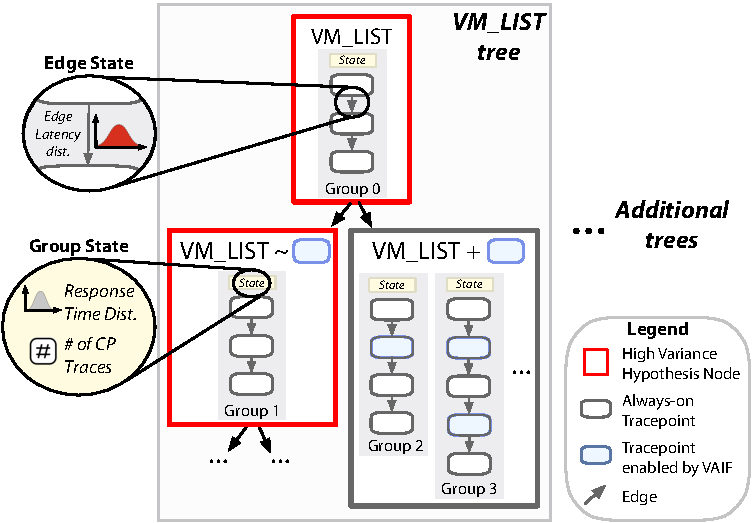
\includegraphics[width=\columnwidth]{figures/hypo.pdf}
 
  \caption{\STAIF{}'s hypothesis forest. This figure shows a \textsc{VM\_LIST} tree from the forest}
  \label{fig:hyp_tree}
   
\end{figure}
}

Figure~\ref{fig:hyp_tree} shows an example hypothesis forest.  Each
tree in the forest encodes hypotheses made on behalf of a different
request type or endpoint that \STAIF{} is initialized with (e.g.,
OpenStack's \textsc{VM\_LIST} in the figure).  This reflects the
intuition that request type is a basic predictor of performance and
that different request types may experience different problems
that benefit from different tracepoints.



Nodes of hypothesis trees (hypothesis nodes) contain pointers to the
results of applying hypotheses. Hypotheses result in two
nodes, one for traces that include the enabled tracepoint and the other
for ones in which it is absent.  Each node includes a field that
names the hypothesis tracepoint and whether it should be present or
absent from traces (e.g., $+$
\includegraphics[scale=0.7, trim=-0 0.1cm 0 0]{figures/blue_bubble.pdf} or $\sim$ 
\includegraphics[scale=0.7, trim=-0 0.1cm 0 0]{figures/blue_bubble.pdf} in the
figure).  The root node of each tree shows results for traces that
include the request-type start tracepoint.

Results are: 1) groups of identical critical-path
traces that either include or exclude the tracepoint and 2) any keys
in included tracepoints that explain variance.  Groups store important
performance information needed for \STAIF{}'s analyses--a
representative trace, response-time distributions of requests assigned
to them, trace edge-latency distributions, and the number of requests
assigned to each group.  Tracepoints enabled by \STAIF{} on behalf of
other paths or trees are removed from traces before grouping.  Such
processing allows \STAIF{} to measure the effects of each hypothesis
independently w/o interference from other hypotheses.  Always-on
tracepoints are not removed as \STAIF{} does not make hypotheses about
them.

\mert{Removed control logic pseudo code and walkthrough. We already talked about control logic so far in high level.}

\subsection{Search space \& search strategies}
\label{sec:design:search_strategies}

\noindent\textbf{Search space} The search space contains: 1) potential
critical paths in requests' workflows when all tracepoints are
enabled; 2) tracepoints that demarcate concurrency or
synchronization; 3) keys within tracepoints that should be
incorporated in grouping and bin ranges for them. % (needed for $search.key\_value()$).   %MERT: there is no search.augment
% All tracepoints are labeled with whether they are always on. % MERT: do we really need to say this
  % (which we assume is a key/value pair).  
Search strategies use the search space to suggest the next tracepoint to
enable between high-variance or -latency trace edges.  %(i.e., $search.find()$)
This requires \textit{matching} the group
critical-path trace representative against potential critical paths in
the search space to determine which path it is most likely to be.

\textit{Potential critical paths:} These are learned by
running exhaustive workloads against the application with all
tracepoints enabled. For traces with multiple
concurrent branches, each unique path within them is stored separately as a
potential critical path. We expect potential critical paths will be
learned as part of organizations' code or coverage tests.  These tests
can be run when deploying an application or updating it.  
\STAIF{} will still provide value if the paths stored in the
search space are incomplete.

\textit{Developer-specified keys and bin ranges:} These are stored as
key name, tracepoint to which they belong, and a set
of bin ranges.  We expect developers will specify only a few select
keys (e.g., ones that correspond to request sizes or ones that
indicate queue lengths for a highly-contended resource.)

\textit{Concurrency / synchronization points:}
These are identified automatically as fan-out and fan-in points in
learned paths.

\textit{Matching to potential critical paths:} For a given group, we transform
its representative trace into a regular expression.  
For example, the trace ``\texttt{A->B->C}'' is
transformed into ``\texttt{.*A.*B.*C.*}''.  The
expression is applied to all potential critical paths to identify
potential matches.  
% MERT: following is removed for trimming
% False matches that include always-on tracepoints that are not contained the group representative trace are discarded.
We choose among multiple matching potential critical paths randomly
\textcolor{red}{(weighted by frequency of their occurrence during learning)}.


%strategy iterates the paths in the search space concurrently. For any
%node (tracepoint) in the group representative, it iterates the
%potential critical paths until an identical node is found. More
%formally, the group representative path ``\texttt{ABC}'' is
%transformed into the regular expression ``\texttt{.*A.*B.*C.*}''.  We
%choose among multiple matching potential critical paths randomly
%weighted by frequency of their occurrence during learning.

\noindent\textbf{Search strategies} The two search strategies either
use the hierarchical or happens-before edges in traces.

% \raja{This is too simple...we did something about areas between spans.}

\textit{Hierarchical search}: This strategy
uses hierarchical edges (called spans in
OpenTelemetry~\cite{opentelemetry}).  Given a pair of tracepoints
that denote a hierarchical level (a span), this strategy determines
which pair of tracepoints (subspan) to enable next.  In the case where
there are multiple subspans, we use binary search to pick the middle
one.

\textit{Flat search:} This strategy uses only
the happens-before relationships.  Given a pair of tracepoints, this
picks a tracepoint that occurs between them.
Tracepoints are ordered by happens-before
relationships and binary search is used to pick among them.


\mert{
  1) Removed Limitations. 2)
}



%-------------------------------------------------------------------------------
\section{How VAIF can help?}
%-------------------------------------------------------------------------------

\mert{Removed all experiments. Only kept intro paragraph below and three case studies from openstack}

\staif{} serves as a fundamental step for developers to
diagnose performance problems, localizing them to a specific area of
the system.  We envision that developers will use \staif{} in two ways;
1) match anomalous traces (e.g., slow requests) to the hypothesis
forest to figure out the performance hypotheses, 2) query the
hypothesis forest by the request type to inquire about the sources of
performance problems.

\textcolor{red}{
This section presents three different case studies of how we used \STAIF{} to
identify various performance problems in OpenStack. Openstack is a widely-used distributed application for
managing clouds.  We use the OpenStack Stein release.  Our cluster
consists of 9 Compute and 1 Controller node.}

\noindent\textbf{Unpredictable performance of \textsc{VM Delete} requests.}
In OpenStack, instances can be deleted using the \textsc{VM Delete} command. 
We find that some \textsc{VM Delete} requests take 28 seconds, where the mean latency is around 20.
We query the hypothesis forest by the slowest request.
\staif{} finds the delete groups have high CV values (0.18) to begin with.
In exploration of variance, \staif{} enables three tracepoints and 
it localizes the high variance to $unplug\_os\_vif$ function. %with problematic group having CV of $0.12$.
This function constitutes 85\% of the variance and 42\% of response time in this request type.
Our analysis from there leads us to a bug report about the performance of this function (\cite{vifplug1,vifplug2}). %, which complains about this library and function.
For this problem, \staif{} helps diagnose a performance
bug due to a delay in a function. 


\noindent\textbf{Lack of instrumentation in the code. }
All instances on OpenStack can be listed using the command \textsc{VM List}.
Matching the slowest trace to the hypothesis forest shows that the request’s latency emanates from three edges. 
This trace's group shows high CV ($0.2$), and the enabled tracepoints constitute 63\% of all variance and 60\% of the latency.
We further examine the code corresponding to those three edges and find the following;
1) two edges ($keystone\_post \& get$) correspond to where identity service (keystone) is utilized for authentication token,
2) the third edge corresponds to a function ($get\_all$) that constitutes 2000 LoC and performs numerous DB lookups to get every instance, including deleted ones.
We corroborate these findings in the bug reports (\cite{listslow1,listslow2}),
 which state that {VM List} experiences latency variations due to  a) the token table getting large in identity service, and 
 b) the function not being able to scale well with the number of VMs and users.
In this case, \staif{} helps diagnose performance problems by isolating latency to (1) a specific service and operation and (2) an inefficient function. 
The latter case also provides an insight to developers as inefficient tracing (i.e., more tracepoints can be added to the 2000 LoC).

\noindent\textbf{Explaining the variance with key/value pairs.}  
% We re-inject the resource-contention problem described
% in Section ~\ref{sec:motivation:guiding_principles}.  
% We re-inject a problem to show how \staif{} can help debug a resource contation issues.
In OpenStack \textsc{VM\_CREATE} requests finish creating new OpenStack VMs very slowly. 
The root cause is that the
number of concurrent servers that can be created within OpenStack's Nova Service is limited to ten by default. 
Additional \textsc{VM\_CREATE} requests are forced to wait on a semaphore.

\staif{} finds that \textsc{VM Create} groups have high CV ($0.21$) initially.
\staif{} finds that the highest-variance edge constitutes
$96\%$ of the variance and 73\% of the response time.  The first
tracepoint of the highest variance edge ($\_build\_semaphore\_start$)
is where a nova-compute manager semaphore is acquired.
Further, \staif{} finds a high correlation between a key/value pair
exposed by the tracepoint (i.e., the number of simultaneous VM
creations) and request's latency (R=$0.85$ w/ p-val $10^{-5}$).

%-------------------------------------------------------------------------------
\section*{Acknowledgments}
%-------------------------------------------------------------------------------

The USENIX latex style is old and very tired, which is why
there's no \textbackslash{}acks command for you to use when
acknowledging. Sorry.

%-------------------------------------------------------------------------------
\bibliographystyle{plain}
\bibliography{\jobname}

%%%%%%%%%%%%%%%%%%%%%%%%%%%%%%%%%%%%%%%%%%%%%%%%%%%%%%%%%%%%%%%%%%%%%%%%%%%%%%%%
\end{document}
%%%%%%%%%%%%%%%%%%%%%%%%%%%%%%%%%%%%%%%%%%%%%%%%%%%%%%%%%%%%%%%%%%%%%%%%%%%%%%%%

%%  LocalWords:  endnotes includegraphics fread ptr nobj noindent
%%  LocalWords:  pdflatex acks
